\documentclass[11pt,openany,a4paper]{article}
\usepackage{amsmath, amsfonts, amssymb, amsthm}
\usepackage{tikz, pgfplots, tkz-euclide,calc}
    \usetikzlibrary{patterns,snakes,shapes.arrows,arrows.meta}
\usepackage{fancyhdr}
\usepackage{enumerate,enumitem}
\usepackage{cancel}
\usepackage{varwidth}
\usepackage{array}
\usepackage{animate}
\usepackage{multirow,multicol}
\usepackage{hyperref}
\hypersetup{
    colorlinks=true,
    linkcolor=blue,
    filecolor=magenta,      
    urlcolor=cyan,
    pdftitle={Overleaf Example},
    pdfpagemode=FullScreen,
    }
\usepackage{graphicx}
\graphicspath{{D:/Hada Touya/Asisten-things/Asisten Dosen/PPT Kalkulus/Gambar & Logo/}{C:/Users/teoso/OneDrive/Documents/Asisten Dosen & Lab/Asisten Laboratorium/Alpro 1/PPT/Graphicx/}{C:/Users/teoso/OneDrive/Documents/Tugas Kuliah/Template Math Depart/}}

% TAMBAHKAN PACKAGE SENDIRI KALAU KURANG

\usepackage{geometry}
\geometry{
	left = 20mm,
	right = 20mm,
	top = 30mm,
	bottom = 30mm,
}


\pagestyle{fancy}
\fancyhead{}
\fancyfoot{}
\fancyhead[r]{}
\fancyhead[l]{\fbox{\large{\textbf{SKPB - ITS}}}}
\renewcommand{\headrulewidth}{0pt}
\renewcommand{\footrulewidth}{0pt}

\newcommand{\R}{\mathbb{R}}
\newcommand{\N}{\mathbb{N}}
\newcommand{\C}{\mathbb{C}}
\newcommand{\Z}{\mathbb{Z}}
\newcommand{\Q}{\mathbb{Q}}
\newcommand{\cis}{\text{cis}}

\begin{document}

\begin{center}
    {\underline{\textbf{\MakeUppercase{Evaluasi Tengah Semester Bersama Genap 2024/2025}}}}
\end{center}

\begin{center}
    \begin{tabular}{lcl}
        Mata kuliah/SKS & : & Kalkulus 1 ( SM234101 ) / 3 SKS \\
        Hari, Tanggal   & : & Kamis, 17 Oktober 2024          \\
        Waktu           & : & 07.00-08.40 WIB (100 menit)     \\
        Sifat           & : & Tertutup                        \\
        Kelas           & : & 5-12, 101
    \end{tabular}
\end{center}

\noindent\rule{\textwidth}{2.pt}

\setlength{\parindent}{5pt}
\setlength{\parindent}{5pt}
\centering{Tuliskan: Nama, NRP, dan Nomor Kelas pada lembar jawaban Anda.}
\setlength{\parindent}{5pt}
\par \textbf{\small\MakeUppercase{dilarang membawa/menggunakan kalkulator dan alat komunikasi}}
\centering{\textbf{\MakeUppercase{dilarang memberikan/menerima jawaban selama ujian}}}
\par \centering{\textbf{"Setiap tindak kecurangan akan mendapat sanksi akademik."}}
\noindent\rule{\textwidth}{2.pt}

\begin{table}[h]
    \centering
    ETS Mengukur Kemampuan
    \begin{tabular}{|c|m{11cm}|c|c|}
        \hline
        CPL & CPMK                                                                                      & SOAL & BOBOT (\%) \\ \hline
        \multirow{5}{*}{2}
            & CPMK-1 Mampu menyelesaikan persamaan dan pertidaksamaan serta menssketsa grafik persamaan & 1    & 20         \\ \cline{2-4}
            & \multirow{4}{*}{CPMK-2 Mampu menentukan kekontinuan fungsi dan turunannya}                & 2    & 20         \\\cline{3-4}
            &                                                                                           & 3    & 20         \\ \cline{3-4}
            &                                                                                           & 4    & 20         \\ \cline{3-4}
            &                                                                                           & 5    & 20         \\ \hline
    \end{tabular}
\end{table}
{\centering\textbf{SOAL}}
% SOAL DI SINI YAA
\begin{enumerate}
    \item Dapatkan himpunan penyelesaian dari
          \[
              \frac{1}{x+2} < \frac{1}{4-x}.
          \]

    \item Diberikan $f(x) = x^2 + 2,\; x \geq 0$ dan $g(x) = \sqrt{x-3}$.
          \begin{enumerate}
              \item Dapatkan domain $f(x)$ dan $g(x)$.
              \item Dapatkan $(g \circ f)(x)$ dan domain $(g \circ f)(x)$.
          \end{enumerate}

    \item Diketahui $f(x) = x^3 - 2$.
          \begin{enumerate}
              \item Dapatkan $f^{-1}(x)$ beserta domainnya.
              \item Sketsa grafik dari $f(x)$ dan $f^{-1}(x)$ pada satu bidang koordinat.
          \end{enumerate}

    \item Hitunglah $\displaystyle\lim_{x \to -\infty} \frac{\sqrt{5x^2 - 2}}{x+3}$.

    \item Dapatkan persamaan garis singgung kurva $xy^2 + y + \sqrt{x} = x + 3$ di titik $(4,1)$.
\end{enumerate}

\fancyfoot{\begin{center}
        \rule{0.28\textwidth}{2.pt}$\quad$\textbf{Selamat Mengerjakan}$\quad$\rule{0.28\textwidth}{2.pt}
        \begin{quote}
            \centering
            \textit{``Jujur adalah kunci kesuksesan''}
        \end{quote}
    \end{center}}


\newpage
\fancyhead[L]{\textit{Solution By: \hyperlink{https://github.com/TetewHeroez}{Tetew}}}
% \fancyfoot[R]{\animategraphics[autoplay,loop,width=0.1\textwidth]{15}{Kuru Kuru Herta/kuru kuru-}{0}{5}}
{\centering\textbf{SOLUSI}}
\renewcommand{\arraystretch}{1.5}
\renewcommand{\headrulewidth}{1pt}
\begin{enumerate}
    \item \begin{align*}
              \frac{1}{x+2}-\frac{1}{4-x}         & < 0 \\
              \iff \frac{4-x - (x+2)}{(x+2)(4-x)} & < 0 \\
              \iff \frac{2 - 2x}{(x+2)(4-x)}      & < 0 \\
              \iff \frac{1-x}{(x+2)(4-x)}         & < 0
          \end{align*}
          Diperoleh pembuat nol $x = 1, -2, 4$.\\
          Selanjutnya gunakan uji tanda, didapatkan
          \begin{itemize}
              \item $x=-3 \implies \frac{1-(-3)}{(-3+2)(4-(-3))} = \frac{4}{-7} < 0$
              \item $x=0 \implies \frac{1-0}{(0+2)(4-0)} = \frac{1}{8} > 0$
              \item $x=2 \implies \frac{1-2}{(2+2)(4-2)} = \frac{-1}{8} < 0$
          \end{itemize}
          \begin{center}
              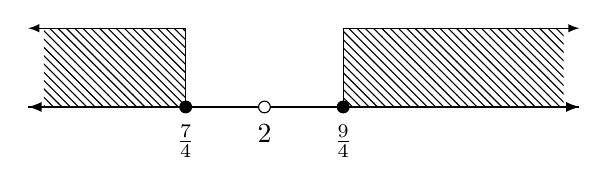
\begin{tikzpicture}
                  \draw[-Latex] (-1,0) -- (6,0);
                  \draw[Latex-] (-1,0) -- (6,0);
                  \foreach \i in {1,2,3}
                  \coordinate (A\i) at (\i,0);
                  \node[below] at ($(0,-0.1)+(A1)$) {$\frac{7}{4}$};
                  \node[below] at ($(0,-0.1)+(A2)$) {$2$};
                  \node[below] at ($(0,-0.1)+(A3)$) {$\frac{9}{4}$};

                  \fill[lightgray,pattern=north west lines,line width=1pt](A1)rectangle($(-0.8,0)+(0,1)$);
                  \fill[lightgray,pattern=north west lines,line width=1pt](A3)rectangle($(5.8,0)+(0,1)$);

                  \draw[-latex](A1)--($(A1)+(0,1)$)--($(-1,0)+(0,1)$);
                  \draw[-latex](A3)--($(A3)+(0,1)$)--($(6,0)+(0,1)$);

                  \foreach \i in {1,3}
                  \node[circle,draw,fill=black,inner sep=1.5pt] at (A\i) {};
                  \node[circle,draw,fill=white,inner sep=1.5pt] at (A2) {};

              \end{tikzpicture}
          \end{center}

\end{enumerate}

\newpage
\renewcommand{\arraystretch}{1}
\fancyhead{}
\fancyfoot{}
\fancyhead[r]{}
\fancyhead[l]{\fbox{\large{\textbf{SKPB - ITS}}}}
\renewcommand{\headrulewidth}{0pt}
\renewcommand{\footrulewidth}{0pt}
\begin{center}
    {\underline{\textbf{\MakeUppercase{Evaluasi Tengah Semester Bersama Genap 2024/2025}}}}
\end{center}

\begin{center}
    \begin{tabular}{lcl}
        Mata kuliah/SKS & : & Kalkulus 1 ( SM234101 ) / 3 SKS \\
        Hari, Tanggal   & : & Kamis, 17 Oktober 2024          \\
        Waktu           & : & 07.00-08.40 WIB (100 menit)     \\
        Sifat           & : & Tertutup                        \\
        Kelas           & : & 13-19, 103
    \end{tabular}
\end{center}

\noindent\rule{\textwidth}{2.pt}

\setlength{\parindent}{5pt}
\setlength{\parindent}{5pt}
\centering{Tuliskan: Nama, NRP, dan Nomor Kelas pada lembar jawaban Anda.}
\setlength{\parindent}{5pt}
\par \textbf{\small\MakeUppercase{dilarang membawa/menggunakan kalkulator dan alat komunikasi}}
\centering{\textbf{\MakeUppercase{dilarang memberikan/menerima jawaban selama ujian}}}
\par \centering{\textbf{"Setiap tindak kecurangan akan mendapat sanksi akademik."}}
\noindent\rule{\textwidth}{2.pt}

\begin{table}[h]
    \centering
    ETS Mengukur Kemampuan
    \begin{tabular}{|c|m{11cm}|c|c|}
        \hline
        CPL & CPMK                                                                                      & SOAL & BOBOT (\%) \\ \hline
        \multirow{5}{*}{2}
            & CPMK-1 Mampu menyelesaikan persamaan dan pertidaksamaan serta menssketsa grafik persamaan & 1    & 20         \\ \cline{2-4}
            & \multirow{4}{*}{CPMK-2 Mampu menentukan kekontinuan fungsi dan turunannya}                & 2    & 20         \\\cline{3-4}
            &                                                                                           & 3    & 20         \\ \cline{3-4}
            &                                                                                           & 4    & 20         \\ \cline{3-4}
            &                                                                                           & 5    & 20         \\ \hline
    \end{tabular}
\end{table}
{\centering\textbf{SOAL}}
% SOAL DI SINI YAA
\begin{enumerate}
    \item Diberikan titik $A(2,-1)$, $B(2,2)$ dan $C(0,4)$. Dapatkan persamaan garis yang melalui titik $A$ dan sejajar dengan garis yang melalui $B$ dan $C$.

    \item Diberikan $f(x) = \dfrac{1}{x^2 - 4}$ dan $g(x) = \sqrt{x+1}$.
          \begin{enumerate}
              \item Dapatkan domain $f(x)$ dan $g(x)$.
              \item Dapatkan $(f \circ g)(x)$ dan domain $(f \circ g)(x)$.
          \end{enumerate}

    \item Diberikan $f(x) = x^2 - 4x + 7$.
          \begin{enumerate}
              \item Tentukan domain dari $f$ sehingga $f^{-1}$ ada.
              \item Dapatkan $f^{-1}$ beserta domainnya.
          \end{enumerate}

    \item Dapatkan nilai $k$ sedemikian sehingga fungsi
          \[
              f(x) =
              \begin{cases}
                  x^2 - k, & x < 3    \\
                  3x - 3,  & x \geq 3
              \end{cases}
          \]
          kontinu di $x=3$.

    \item Dapatkan $f'(x)$ dimana
          $
              f(x) = \sqrt{\dfrac{(3x+1)^3}{2x}}.
          $

\end{enumerate}

\fancyfoot{\begin{center}
        \rule{0.28\textwidth}{2.pt}$\quad$\textbf{Selamat Mengerjakan}$\quad$\rule{0.28\textwidth}{2.pt}
        \begin{quote}
            \centering
            \textit{``Jujur adalah kunci kesuksesan''}
        \end{quote}
    \end{center}}


\newpage
\fancyhead[L]{\textit{Solution By: \hyperlink{https://github.com/TetewHeroez}{Tetew}}}
% \fancyfoot[R]{\animategraphics[autoplay,loop,width=0.1\textwidth]{15}{Kuru Kuru Herta/kuru kuru-}{0}{5}}
{\centering\textbf{SOLUSI}}
\renewcommand{\arraystretch}{1.5}
\renewcommand{\headrulewidth}{1pt}
\begin{enumerate}
    \item
\end{enumerate}

\newpage
\renewcommand{\arraystretch}{1}
\fancyhead{}
\fancyfoot{}
\fancyhead[r]{}
\fancyhead[l]{\fbox{\large{\textbf{SKPB - ITS}}}}
\renewcommand{\headrulewidth}{0pt}
\renewcommand{\footrulewidth}{0pt}
\begin{center}
    {\underline{\textbf{\MakeUppercase{Evaluasi Tengah Semester Bersama Genap 2024/2025}}}}
\end{center}

\begin{center}
    \begin{tabular}{lcl}
        Mata kuliah/SKS & : & Kalkulus 1 ( SM234101 ) / 3 SKS \\
        Hari, Tanggal   & : & Kamis, 17 Oktober 2024          \\
        Waktu           & : & 11.00-12.40 WIB (100 menit)     \\
        Sifat           & : & Tertutup                        \\
        Kelas           & : & 20-33, 105, 106
    \end{tabular}
\end{center}

\noindent\rule{\textwidth}{2.pt}

\setlength{\parindent}{5pt}
\setlength{\parindent}{5pt}
\centering{Tuliskan: Nama, NRP, dan Nomor Kelas pada lembar jawaban Anda.}
\setlength{\parindent}{5pt}
\par \textbf{\small\MakeUppercase{dilarang membawa/menggunakan kalkulator dan alat komunikasi}}
\centering{\textbf{\MakeUppercase{dilarang memberikan/menerima jawaban selama ujian}}}
\par \centering{\textbf{"Setiap tindak kecurangan akan mendapat sanksi akademik."}}
\noindent\rule{\textwidth}{2.pt}

\begin{table}[h]
    \centering
    ETS Mengukur Kemampuan
    \begin{tabular}{|c|m{11cm}|c|c|}
        \hline
        CPL & CPMK                                                                                      & SOAL & BOBOT (\%) \\ \hline
        \multirow{5}{*}{2}
            & CPMK-1 Mampu menyelesaikan persamaan dan pertidaksamaan serta menssketsa grafik persamaan & 1    & 20         \\ \cline{2-4}
            & \multirow{4}{*}{CPMK-2 Mampu menentukan kekontinuan fungsi dan turunannya}                & 2    & 20         \\\cline{3-4}
            &                                                                                           & 3    & 20         \\ \cline{3-4}
            &                                                                                           & 4    & 20         \\ \cline{3-4}
            &                                                                                           & 5    & 20         \\ \hline
    \end{tabular}
\end{table}
{\centering\textbf{SOAL}}
% SOAL DI SINI YAA
\begin{enumerate}
    \item Dapatkan himpunan penyelesaian dari
          \[
              -1 \leq |2 - x| < 3.
          \]

    \item Diberikan $f(x) = \sqrt{25 - x^2}$ dan $g(x) = \dfrac{1}{x^2}$.
          \begin{enumerate}
              \item Dapatkan domain $f(x)$ dan $g(x)$.
              \item Dapatkan $(g \circ f)(x)$ dan domain $(g \circ f)(x)$.
          \end{enumerate}

    \item Diberikan $f(x) = \sqrt{4 - x^2}$.
          \begin{enumerate}
              \item Tentukan domain dari $f(x)$ sehingga inversnya ada.
              \item Dapatkan $f^{-1}(x)$ beserta domainnya.
          \end{enumerate}

    \item Diberikan fungsi
          \[
              f(x) =
              \begin{cases}
                  \dfrac{4 - x}{2 - \sqrt{x}}, & x \neq 4, \\[1em]
                  6,                           & x = 4,
              \end{cases}
          \]
          selidiki kekontinuan $f(x)$ di $x = 4$.

    \item Dapatkan $f''(x)$ dimana
          $
              f(x) = 2x + \bigl( 2\sqrt{x} - 3 \bigr)^{-2}.
          $

\end{enumerate}

\fancyfoot{\begin{center}
        \rule{0.28\textwidth}{2.pt}$\quad$\textbf{Selamat Mengerjakan}$\quad$\rule{0.28\textwidth}{2.pt}
        \begin{quote}
            \centering
            \textit{``Jujur adalah kunci kesuksesan''}
        \end{quote}
    \end{center}}


\newpage
\fancyhead[L]{\textit{Solution By: \hyperlink{https://github.com/TetewHeroez}{Tetew}}}
% \fancyfoot[R]{\animategraphics[autoplay,loop,width=0.1\textwidth]{15}{Kuru Kuru Herta/kuru kuru-}{0}{5}}
{\centering\textbf{SOLUSI}}
\renewcommand{\arraystretch}{1.5}
\renewcommand{\headrulewidth}{1pt}
\begin{enumerate}
    \item
\end{enumerate}

\newpage
\renewcommand{\arraystretch}{1}
\fancyhead{}
\fancyfoot{}
\fancyhead[r]{}
\fancyhead[l]{\fbox{\large{\textbf{SKPB - ITS}}}}
\renewcommand{\headrulewidth}{0pt}
\renewcommand{\footrulewidth}{0pt}
\begin{center}
    {\underline{\textbf{\MakeUppercase{Evaluasi Tengah Semester Bersama Genap 2024/2025}}}}
\end{center}

\begin{center}
    \begin{tabular}{lcl}
        Mata kuliah/SKS & : & Kalkulus 1 ( SM234101 ) / 3 SKS \\
        Hari, Tanggal   & : & Kamis, 17 Oktober 2024          \\
        Waktu           & : & 13.30-15.10 WIB (100 menit)     \\
        Sifat           & : & Tertutup                        \\
        Kelas           & : & 34-46, 107, 108
    \end{tabular}
\end{center}

\noindent\rule{\textwidth}{2.pt}

\setlength{\parindent}{5pt}
\setlength{\parindent}{5pt}
\centering{Tuliskan: Nama, NRP, dan Nomor Kelas pada lembar jawaban Anda.}
\setlength{\parindent}{5pt}
\par \textbf{\small\MakeUppercase{dilarang membawa/menggunakan kalkulator dan alat komunikasi}}
\centering{\textbf{\MakeUppercase{dilarang memberikan/menerima jawaban selama ujian}}}
\par \centering{\textbf{"Setiap tindak kecurangan akan mendapat sanksi akademik."}}
\noindent\rule{\textwidth}{2.pt}

\begin{table}[h]
    \centering
    ETS Mengukur Kemampuan
    \begin{tabular}{|c|m{11cm}|c|c|}
        \hline
        CPL & CPMK                                                                                      & SOAL & BOBOT (\%) \\ \hline
        \multirow{5}{*}{2}
            & CPMK-1 Mampu menyelesaikan persamaan dan pertidaksamaan serta menssketsa grafik persamaan & 1    & 20         \\ \cline{2-4}
            & \multirow{4}{*}{CPMK-2 Mampu menentukan kekontinuan fungsi dan turunannya}                & 2    & 20         \\\cline{3-4}
            &                                                                                           & 3    & 20         \\ \cline{3-4}
            &                                                                                           & 4    & 20         \\ \cline{3-4}
            &                                                                                           & 5    & 20         \\ \hline
    \end{tabular}
\end{table}
{\centering\textbf{SOAL}}
% SOAL DI SINI YAA
\begin{enumerate}
    \item Diberikan titik $A(1,1)$, $B(4,2)$ dan $C(2,6)$. Tentukan jarak dari titik $C$ ke garis yang melalui titik $A$ dan $B$.

    \item Diberikan $f(x) = x - 4$, untuk $x \geq 4$ dan $g(x) = \sqrt{4 - x^2}$.
          \begin{enumerate}
              \item Dapatkan domain $f(x)$ dan $g(x)$.
              \item Tentukan $(g \circ f)(x)$ dan domain $(g \circ f)(x)$.
          \end{enumerate}

    \item Diberikan fungsi $f(x) = \sqrt{2x - x^2}, \; 0 \leq x \leq 1$.
          \begin{enumerate}
              \item Tentukan $f^{-1}(x)$ beserta domainnya.
              \item Gambarkan grafik $f(x)$ dan $f^{-1}(x)$ dalam satu bidang koordinat.
          \end{enumerate}

    \item Hitunglah
          $\displaystyle
              \lim_{x \to 2} \frac{\sqrt{x^2 + 5} - 3}{x - 2}.
          $

    \item Diketahui persamaan garis singgung kurva $y^2 - xy = -2$ di titik $(a,b)$ sejajar dengan kurva $y = -x$.
          Dapatkan titik $(a,b)$.

\end{enumerate}

\fancyfoot{\begin{center}
        \rule{0.28\textwidth}{2.pt}$\quad$\textbf{Selamat Mengerjakan}$\quad$\rule{0.28\textwidth}{2.pt}
        \begin{quote}
            \centering
            \textit{``Jujur adalah kunci kesuksesan''}
        \end{quote}
    \end{center}}


\newpage
\fancyhead[L]{\textit{Solution By: \hyperlink{https://github.com/TetewHeroez}{Tetew}}}
% \fancyfoot[R]{\animategraphics[autoplay,loop,width=0.1\textwidth]{15}{Kuru Kuru Herta/kuru kuru-}{0}{5}}
{\centering\textbf{SOLUSI}}
\renewcommand{\arraystretch}{1.5}
\renewcommand{\headrulewidth}{1pt}
\begin{enumerate}
    \item
\end{enumerate}

\newpage
\renewcommand{\arraystretch}{1}
\fancyhead{}
\fancyfoot{}
\fancyhead[r]{}
\fancyhead[l]{\fbox{\large{\textbf{SKPB - ITS}}}}
\renewcommand{\headrulewidth}{0pt}
\renewcommand{\footrulewidth}{0pt}
\begin{center}
    {\underline{\textbf{\MakeUppercase{Evaluasi Tengah Semester Bersama Genap 2024/2025}}}}
\end{center}

\begin{center}
    \begin{tabular}{lcl}
        Mata kuliah/SKS & : & Kalkulus 1 ( SM234101 ) / 3 SKS \\
        Hari, Tanggal   & : & Kamis, 17 Oktober 2024          \\
        Waktu           & : & 09.00-10.40 WIB (100 menit)     \\
        Sifat           & : & Tertutup                        \\
        Kelas           & : & 47-59, 111
    \end{tabular}
\end{center}

\noindent\rule{\textwidth}{2.pt}

\setlength{\parindent}{5pt}
\setlength{\parindent}{5pt}
\centering{Tuliskan: Nama, NRP, dan Nomor Kelas pada lembar jawaban Anda.}
\setlength{\parindent}{5pt}
\par \textbf{\small\MakeUppercase{dilarang membawa/menggunakan kalkulator dan alat komunikasi}}
\centering{\textbf{\MakeUppercase{dilarang memberikan/menerima jawaban selama ujian}}}
\par \centering{\textbf{"Setiap tindak kecurangan akan mendapat sanksi akademik."}}
\noindent\rule{\textwidth}{2.pt}

\begin{table}[h]
    \centering
    ETS Mengukur Kemampuan
    \begin{tabular}{|c|m{11cm}|c|c|}
        \hline
        CPL & CPMK                                                                                      & SOAL & BOBOT (\%) \\ \hline
        \multirow{5}{*}{2}
            & CPMK-1 Mampu menyelesaikan persamaan dan pertidaksamaan serta menssketsa grafik persamaan & 1    & 20         \\ \cline{2-4}
            & \multirow{4}{*}{CPMK-2 Mampu menentukan kekontinuan fungsi dan turunannya}                & 2    & 20         \\\cline{3-4}
            &                                                                                           & 3    & 20         \\ \cline{3-4}
            &                                                                                           & 4    & 20         \\ \cline{3-4}
            &                                                                                           & 5    & 20         \\ \hline
    \end{tabular}
\end{table}
{\centering\textbf{SOAL}}
% SOAL DI SINI YAA
\begin{enumerate}
    \item Dapatkan himpunan penyelesaian dari
          $\displaystyle
              \frac{x}{|2x - 5|} > 5.
          $

    \item Diberikan $f(x) = \sqrt{x - 3}$ dan $g(x) = 1 + \sqrt{x - 5}$.
          \begin{enumerate}
              \item Dapatkan domain $f(x)$ dan $g(x)$.
              \item Dapatkan $(f \circ g)(x)$ dan domain $(f \circ g)(x)$.
          \end{enumerate}

    \item Diberikan $f(x) = \sqrt[3]{x} - 1, \; x \geq 1$.
          \begin{enumerate}
              \item Dapatkan $f^{-1}(x)$ beserta domainnya.
              \item Sketsa $f(x)$ dan $f^{-1}(x)$ pada satu bidang koordinat.
          \end{enumerate}

    \item Hitunglah
          $\displaystyle
              \lim_{y \to \infty} \frac{2 - y}{\sqrt{7 + 4y^2}}.
          $

    \item Dapatkan persamaan garis singgung kurva
          $
              x^2 + y + \frac{y}{x} = \sqrt{x} + 2
          $
          di titik $(1,1)$.
\end{enumerate}


\fancyfoot{\begin{center}
        \rule{0.28\textwidth}{2.pt}$\quad$\textbf{Selamat Mengerjakan}$\quad$\rule{0.28\textwidth}{2.pt}
        \begin{quote}
            \centering
            \textit{``Jujur adalah kunci kesuksesan''}
        \end{quote}
    \end{center}}


\newpage
\fancyhead[L]{\textit{Solution By: \hyperlink{https://github.com/TetewHeroez}{Tetew}}}
% \fancyfoot[R]{\animategraphics[autoplay,loop,width=0.1\textwidth]{15}{Kuru Kuru Herta/kuru kuru-}{0}{5}}
{\centering\textbf{SOLUSI}}
\renewcommand{\arraystretch}{1.5}
\renewcommand{\headrulewidth}{1pt}
\begin{enumerate}
    \item
\end{enumerate}
\end{document}